
\subsubsection{25.10.14}

\begin{enumerate}
	\item The time of beginning and ending of the congregation:
	16:00 - 20:00
	\item Purposes of the congregation:
	\begin{enumerate}
	  \item To elaborate and create the mechanism of capture movable baskets. 
	  
    \end{enumerate}
    
	\item Work, that has been done:
	\begin{enumerate}
	  \item It was considered 2 options of mechanism of capture movable baskets (hereinafter it will be called MCB):
	  \begin{enumerate}
	    \item Servo at which fixed the beam. When servo rotates beam turns and lowers.
	    
	    \item To the rear edge of robot is fixed  the furniture slat which connected with servo with help fishing line. When servo rotates, slat lowers.
	    
	    \begin{figure}[H]
	    	\begin{minipage}[h]{0.2\linewidth}
	    		\center   
	    	\end{minipage}
	    	\begin{minipage}[h]{0.6\linewidth}
	    		\center{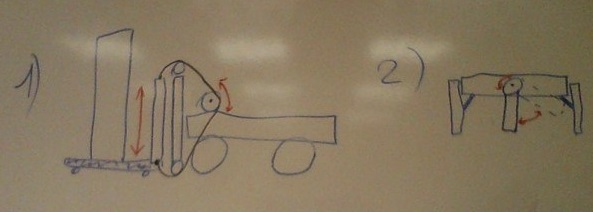
\includegraphics[scale=0.55]{days/25.10.14/images/01}}
	    		\caption{Ideas of MCB 1)Slat 2)Servo with beam}
	    	\end{minipage}
	    \end{figure}
	    
      \end{enumerate}
      \item It was decided to make MCB with slat because this variant more compact.
      
      \item The furniture slat was sawn for reduce its length.
      
      \begin{figure}[H]
      	\begin{minipage}[h]{0.2\linewidth}
      		\center   
      	\end{minipage}
      	\begin{minipage}[h]{0.6\linewidth}
      		\center{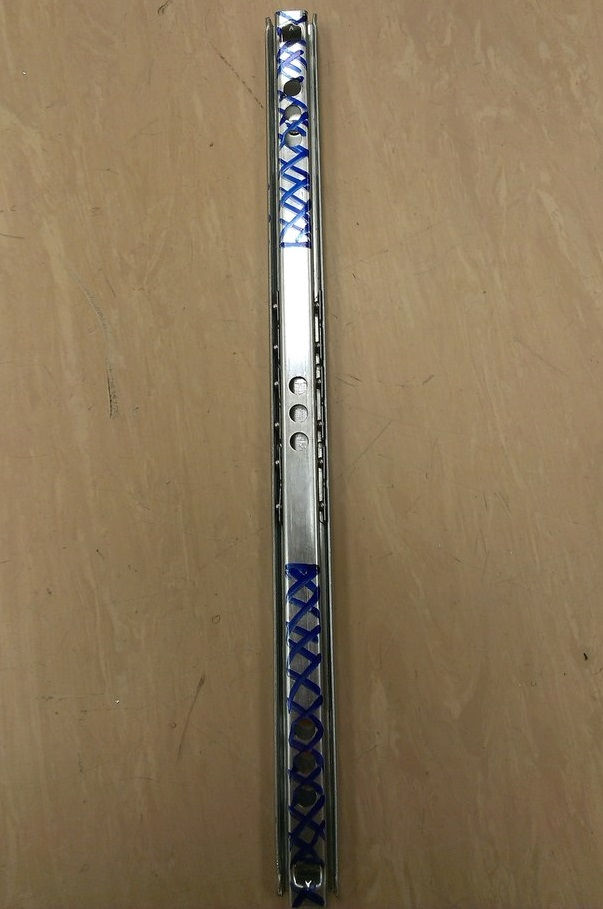
\includegraphics[scale=0.24]{days/25.10.14/images/02}}
      		\caption{Shortened furniture slat \newline (the sawn part is hatched)}
      	\end{minipage}
      \end{figure}
      
      \item On the slat were marked location for drilling holes for mounts. The holes weren't drilled because we didn't have the drill.
      
    \end{enumerate}
    
	\item Results: 
	\begin{enumerate}
	  \item MCB was elaborated but didn't installed.
      
    \end{enumerate}
    
	\item Tasks for the next congregations:
	\begin{enumerate}
	  \item Finish creating of MCB.
	  
    \end{enumerate}     
\end{enumerate}
\fillpage
